\section{Memory Decomposition Abstraction}


\nt{read and include \cite{Catanzaro2009} it is about Productivity language JIT compilation into efficient language
And get all the paper that cite this one.
}
\nt{read and include \cite{Engler1994}}

\nt{read and include \cite{Kovachev2011}}


\subsection{Runtime}

The criteria to analyze the solutions presented in this section are :
\begin{itemize}
\item criteria 1
\item criteria 2
\end{itemize}


\begin{figure}[h!]
\begin{center}
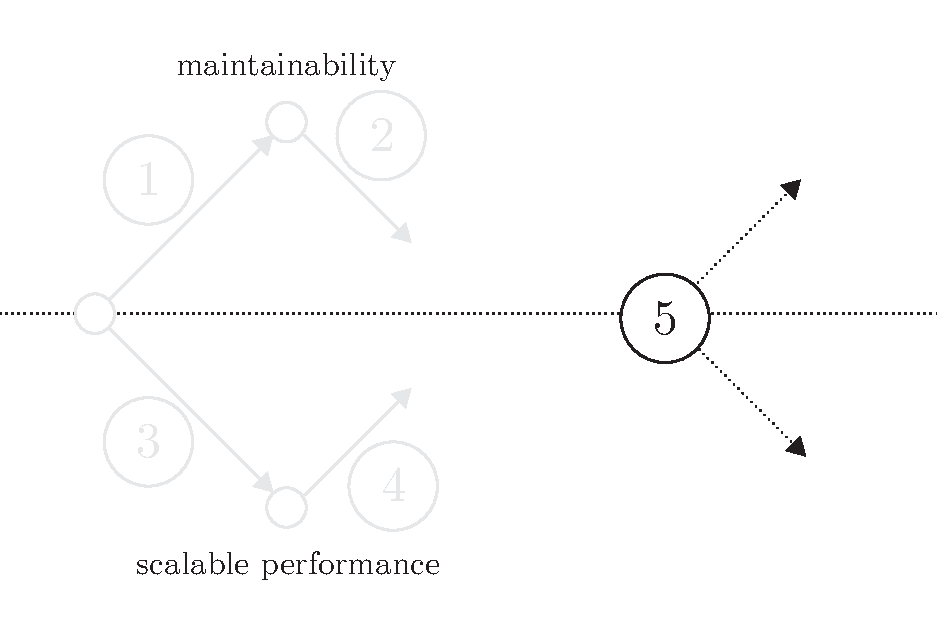
\includegraphics[width=0.6\textwidth]{../ressources/state-of-the-art-5.pdf}
\end{center}
\end{figure}





\subsubsection{Partitioned Global Address Space}

Parallelization of the execution eventually requires the distribution of the memory.
The Partitioned Global Address Space (PGAS) provides the developers with a uniform memory access on a distributed architecture.
It attempts to combine the advantage of SPMD programming style for distributed memory systems, with the data referencing semantics of shared memory systems.
Each computing node executes the same program, and provide its local memory to be shared with all the other nodes.
The PGAS programming model assure the remote accesses and synchronization of memory across nodes, and enforces locality of reference, to reduce the communication overhead.
Examples of implementation of the PGAS model are 
CoArray Fortran \cite{Numrich1998},
X10 \cite{Charles2005}.
Unified Parallel C \cite{El-Ghazawi2006},
Chapel\cite{Chamberlain2007},
OpenSHMEM \cite{Chapman2010}.
Kokko \cite{Edwards2012},
UPC++ \cite{Zheng2014},
RAJA \cite{Hornung2014},
ACPdl \cite{Ajima2015} and
HPX \cite{Kaiser2015}\nt{include as well HPX: A Task Based Programming Model in a Global Address Space by Kaiser, Heller, Adelstein-Lelbach}.

% These programming models are promising.
% However, they focus rather on scientific application with intensive computing such as matrix multiplication, and leave out streaming applications, such as web services.





\subsubsection{Dynamic Distribution of Execution}

An interesting work following SEDA, is Leda \cite{Salmito2013,Salmito2014}.It follows the PCAM design methodology \cite{Foster1995} to propose a model where the stages of the pipeline are defined only by their role in the application.
% Partition $\to$ Communicate $\to$ Agglomerate $\to$ Map.
The actual execution distribution in stages is defined automatically, only after the development, during deployment.
This automation blurs the distinction between the parallel organization of execution, and the modular organization of implementation.
It manages the execution organizations to helps the developer focus on the modular organization.





\subsection{Compilation} \label{chapter3:software-maintainability:performance:compilation}

\cit{It is a mistake to attempt high concurrency without help from the compiler}{R. Behren, J. Condit, E. Brewer \cite{Behren2003}}.

D. Parnas advocates the use of an assembler to conciliate the two approaches \cite{Parnas1972}.

When showing the incompatibility between the two organization, D. Parnas  advocated conciliating the two methods using an assembler to transform the development organization into the execution organization \cite{Parnas1972}.
This section presents the state of the art to extract parallelization from sequential programs through code transformation and compilation.

\nt{read and include \cite{Catanzaro2009}}

\subsubsection{Parallelism Extraction}

As the only requirement to parallelism is the commutativity of operations \cite{Rinard1996,Clements2013a}, a compiler needs to identify the commutative operations transform a sequential program so as to parallelize its execution \cite{Rinard1996}.

An important work was done to parallelize loop iterations \cite{Mauras1989,Amarasinghe1995,Chen2008,Banerjee2013,Radoi2014}, particularly using the polyhedral compilation method \cite{Yuki2013,Grosser2011,Trifunovic2010,Bastoul2004}.
However, this data parallelism is limited to scientific applications because of their heavy use of loops on matrices and vectors.
The performance gains are limited in common sequential programs, as the execution remains sequential outside of loops \cite{Amdahl1967,Clements2013a}.

To improve performance gains further, some compilers identify the data-flow inside sequential programs to allow parallelism on the whole program, and not only on its loops \cite{Beck1991,Catanzaro2009,Li2012}.
Moreover, the data-flow representation and execution of a program is well suited for modern data processing applications \cite{Fernandez2014a}, as well as web services \cite{Salmito2013}.
\nt{TODO Extract parallelism compilers from these :
Load balanced pipeline parallelism \cite{Kamruzzaman2013}, 
Regent \cite{Slaughter2015},
Cilk-P, On-the-Fly Pipeline Parallelism\cite{Lee2013}
}

However, the limitation of modular programming regarding parallelization persists.
In a purely functional language with immutability, higher-order functions are referentially transparent which implies commutativity hence parallelism \nt{Add reference of parallel purely functional languages}.
% \cite{Herrmann2000}
However, in a functional language with mutable data, closures remains a challenge to parallelize, because of the memory references shared across the program \cite{Harrison1989, Nicolay2010, Matsakis2012a}.
The next two paragraphs presents two directions to improve the state of the art in parallel compilation.
The first paragraph presents static analysis, while the second presents annotations systems.

% - Continuation-passing style parallelization compilation \cite{Harrison1989}.The interprocedural analysis and automatic parallelization of Scheme programs
% - Automatic Parallelization of Scheme Programs using Static Analysis \cite{Nicolay2010}

% - Commutativity analysis: A new analysis framework for parallelizing compilers \cite{Rinard1996}
% In this paper, they analyze commutative operations to parallelize them.
% It is novel because it isn't about parallelizing loops.
% However, it is not exactly pipeline parallelism either.

% Introducing 'Bones': a parallelizing source-to-source compiler based on algorithmic skeletons \cite{Nugteren2012}

\subsubsection{Static analysis}

% Intermediate representation is Abstract Syntax Tree
% Static Single Assignment Form \cite{Cytron1991}
% Continuation Passing Style.

Compilers analyze the control-flow of a program to detect the side-effects causing dependencies between statements \cite{Allen1970}.
The point-to analysis, presented by L. Andersen \cite{Andersen1994} is a popular approach to identify these side-effects in the memory representation.
The points-to-analysis was adapted for Javascript \cite{Jang2009,Sridharan2012,Wei2014}, and is a useful tool to analyze a program.
However, this analysis is not sufficient to track the dynamic control-flow of higher-order functions \cite{Shivers1991} like used in Javascript.

The Operational Semantics is an example of abstract interpretation technique that allows to statically reason on the behavior of programs\cite{Maffeis2008,Smith2011,Gardner2012,Gardner2013,Bodin2014}.
\nt{TODO review this paragraph}
Abstract interpretation techniques are more adapted for program with higher-order functions, and are successfully used for security applications \cite{Huang2004,Jovanovic2006,Yu2007,Maffeis2009a,Chudnov2015,Dolby2015}\nt{Update the citation for Dolby2015}.
\nt{Read and include \cite{Hackett2012}}
\nt{Read and include Effective race detection for event-driven programs, by Raychev, Vechev, Sridharan}

However, static analysis techniques are too imprecise, and expensive for the performance gain to be profitable in languages as dynamic as Javascript.
Instead, some compilers relies on annotations from the developers.
% These results suggest that dataflow graphs can serve as an executable intermediate representation in parallel compilers \cite{Beck1991}.

\subsubsection{Annotations}

Extracting parallel dataflow from an imperative, sequential implementation is a hard problem \cite{Johnston2004a}.
Some works proposed to rely on annotations from the developer to help the identify the possible side-effects between operations \cite{Vandierendonck2010a,Fernandez2014a}.
% Some works asked the developers to annotate their code so as help the compiler extract parallelism
% It is an intermediate solution with the solution presented in the previous section.

Many compilers rely on annotations from the developer to build highly parallel executables.
Such annotations are especially relevant for accelerators such as GPUs or FPGAs, because the development effort yield huge performance improvements.
Examples of such compilers are OpenMP \cite{Dagum1998}, OpenCL \cite{Stone2010}, CUDA \cite{Nvidia2007} Cg \cite{Mark2003}, Brook \cite{Buck2004}, Liquid Metal \cite{Huang2008}.

\nt{read and include \cite{Catanzaro2009}}
\nt{read and include Accelerators: Using data parallelism to program gpus for general purpose uses}

However, the burden of detecting commutativity of operations, or independence of operations fall back to the developer.
In this regard, these solutions successfully improve performances, but are unable to fix the rupture between performance and maintainability.
These solutions are indeed very close to the performance oriented solutions presented in the section \ref{chapter3:software-performance}.

% Bloom declarative language \ftnt{http://bloom-lang.net/}
% Blazes: Coordination analysis for distributed programs \cite{Alvaro2014}

% Livescript
% Typescript 
% Annotations, but not for parallelism.
% Asynchronism annotations should be sufficient.

\subsubsection{Compilation Limitations}

The static analysis of static, low level languages like FORTRAN or C, brings performance improvements.
However for more dynamic, higher-level languages like Javascript, the static analysis is not sufficient to identify correctly the dependencies between operations to parallelize them.
And parallel compilers often fall back on relying on annotation provided by developers.
So, in this regards, it seems that the accessibility of development gained by higher-level programming is detrimental to performance.




\begin{table}[h!]
\label{maintainability-scalability}
\small
\begin{tabu} to \linewidth {@{} l X[l] c c c @{}}
%
% \multicolumn{3}{c}{}  & \rot{Concurrency} & \multicolumn{2}{|c}{Parallelism} \\
Model & Implementations    & \rot{Memory decomposition abstraction} & $\to$ & \rot{Maintainability} \\
\tabucline[.5pt]{-}
%                                                                               ABS   MAI
PGAS                           & CoArray Fortran \cite{Numrich1998},
                                 X10 \cite{Charles2005}.
                                 Unified Parallel C \cite{El-Ghazawi2006},
                                 Chapel\cite{Chamberlain2007},
                                 OpenSHMEM \cite{Chapman2010}.
                                 Kokko \cite{Edwards2012},
                                 UPC++ \cite{Zheng2014},
                                 RAJA \cite{Hornung2014},
                                 ACPdl \cite{Ajima2015},
                                 HPX \cite{Kaiser2015}                         & \V && \V \\ \tabucline[on .5pt]{-}
Dynamic distribution           & LEDA                                          & \V && \V \\ \tabucline[on .5pt]{-}
Parallelism extraction         & Polyhedral compiler                           & \V && \V \\ \tabucline[on .5pt]{-}
Annotations                    & OpenMP \cite{Dagum1998},
                                 OpenCL \cite{Stone2010},
                                 CUDA \cite{Nvidia2007} Cg \cite{Mark2003},
                                 Brook \cite{Buck2004},
                                 Liquid Metal \cite{Huang2008}                 & \V && \V \\
\tabucline[.5pt]{-}
\end{tabu}
\caption{Analysis of the state of the art regarding maintainability}
\end{table}




\subsection{Organic Growth}


A system is maintainable only if there is competences available to maintain it.

The criteria to analyze the solutions presented in this section regarding the organic growth are : 
\begin{itemize}
\item adoption by the community
\item adoption by the industry
\item supporting web technologies
\end{itemize}
The first two criteria make sure that the technology is growing organically with a passionate community, and backed by industrial needs.
The last criteria assures the fitting of the technologies with our economical context of a web application. 




\begin{figure}[h!]
\begin{center}
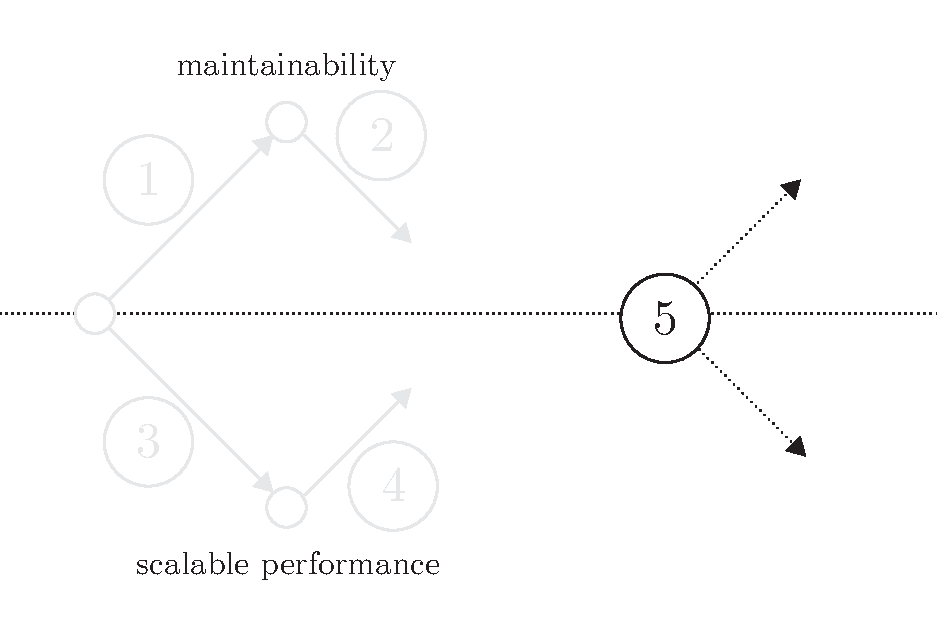
\includegraphics[width=0.6\textwidth]{../ressources/state-of-the-art-5.pdf}
\end{center}
\end{figure}







\begin{table}[h!]
\label{maintainability-scalability}
\small
\begin{tabu} to \linewidth {@{} l X[l] c c c @{}}
%
% \multicolumn{3}{c}{}  & \rot{Concurrency} & \multicolumn{2}{|c}{Parallelism} \\
Model & Implementations    & \rot{Memory decomposition abstraction} & $\to$ & \rot{Maintainability} \\
\tabucline[.5pt]{-}
%                                                                               ABS   MAI
PGAS                           & CoArray Fortran \cite{Numrich1998},
                                 X10 \cite{Charles2005}.
                                 Unified Parallel C \cite{El-Ghazawi2006},
                                 Chapel\cite{Chamberlain2007},
                                 OpenSHMEM \cite{Chapman2010}.
                                 Kokko \cite{Edwards2012},
                                 UPC++ \cite{Zheng2014},
                                 RAJA \cite{Hornung2014},
                                 ACPdl \cite{Ajima2015},
                                 HPX \cite{Kaiser2015}                         & \V && \V \\ \tabucline[on .5pt]{-}
Dynamic distribution           & LEDA                                          & \V && \V \\ \tabucline[on .5pt]{-}
Parallelism extraction         & Polyhedral compiler                           & \V && \V \\ \tabucline[on .5pt]{-}
Annotations                    & OpenMP \cite{Dagum1998},
                                 OpenCL \cite{Stone2010},
                                 CUDA \cite{Nvidia2007} Cg \cite{Mark2003},
                                 Brook \cite{Buck2004},
                                 Liquid Metal \cite{Huang2008}                 & \V && \V \\
\tabucline[.5pt]{-}
\end{tabu}
\caption{Analysis of the state of the art regarding maintainability}
\end{table}



\subsection{Limitations}



To allow a continuous development of a web service, a language must present these three features :

\begin{itemize}
\item scalability
\item maintainability
\item abstract the decomposition
\end{itemize}

The first allows the evolution of the performance.
The second assure the evolution of the implementation.
The third is required to allow these two first features to coexist.




\begin{table}[h!]
\label{maintainability-scalability}
\small
\begin{tabu} to \linewidth {@{} l X[l] c c c @{}}
%
% \multicolumn{3}{c}{}  & \rot{Concurrency} & \multicolumn{2}{|c}{Parallelism} \\
Model & Implementations    & \rot{Memory decomposition abstraction} & $\to$ & \rot{Maintainability} \\
\tabucline[.5pt]{-}
%                                                                               ABS   MAI
PGAS                           & CoArray Fortran \cite{Numrich1998},
                                 X10 \cite{Charles2005}.
                                 Unified Parallel C \cite{El-Ghazawi2006},
                                 Chapel\cite{Chamberlain2007},
                                 OpenSHMEM \cite{Chapman2010}.
                                 Kokko \cite{Edwards2012},
                                 UPC++ \cite{Zheng2014},
                                 RAJA \cite{Hornung2014},
                                 ACPdl \cite{Ajima2015},
                                 HPX \cite{Kaiser2015}                         & \V && \V \\ \tabucline[on .5pt]{-}
Dynamic distribution           & LEDA                                          & \V && \V \\ \tabucline[on .5pt]{-}
Parallelism extraction         & Polyhedral compiler                           & \V && \V \\ \tabucline[on .5pt]{-}
Annotations                    & OpenMP \cite{Dagum1998},
                                 OpenCL \cite{Stone2010},
                                 CUDA \cite{Nvidia2007} Cg \cite{Mark2003},
                                 Brook \cite{Buck2004},
                                 Liquid Metal \cite{Huang2008}                 & \V && \V \\
\tabucline[.5pt]{-}
\end{tabu}
\caption{Analysis of the state of the art regarding maintainability}
\end{table}




\subsection{Summary}



\begin{table}[h!]
\label{maintainability-scalability}
\small
\begin{tabu} to \linewidth {@{} l X[l] c c c @{}}
%
% \multicolumn{3}{c}{}  & \rot{Concurrency} & \multicolumn{2}{|c}{Parallelism} \\
Model & Implementations    & \rot{Modularity} & \rot{Organic Growth} & \rot{Scalability} \\
\tabucline[.5pt]{-}
%                                                                               MOD  GRO  SCA
PGAS                           & CoArray Fortran \cite{Numrich1998},
                                 X10 \cite{Charles2005}.
                                 Unified Parallel C \cite{El-Ghazawi2006},
                                 Chapel\cite{Chamberlain2007},
                                 OpenSHMEM \cite{Chapman2010}.
                                 Kokko \cite{Edwards2012},
                                 UPC++ \cite{Zheng2014},
                                 RAJA \cite{Hornung2014},
                                 ACPdl \cite{Ajima2015},
                                 HPX \cite{Kaiser2015}                         & \V & \X & \V \\ \tabucline[on .5pt]{-}
Dynamic distribution           & LEDA                                          & \V & \X & \V \\ \tabucline[on .5pt]{-}
Parallelism extraction         & Polyhedral compiler                           & \V & \X & \V \\ \tabucline[on .5pt]{-}
Annotations                    & OpenMP \cite{Dagum1998},
                                 OpenCL \cite{Stone2010},
                                 CUDA \cite{Nvidia2007} Cg \cite{Mark2003},
                                 Brook \cite{Buck2004},
                                 Liquid Metal \cite{Huang2008}                 & \V & \X & \V \\
\tabucline[.5pt]{-}
\end{tabu}
\caption{Summary of the analysis of the state of the art}
\end{table}